\chapter{Learning Residual Probabilistic Observation Functions through Error-State Kalman Filters}

\begin{figure}[h!]
    \centering
    \begin{subfigure}[]{0.9\textwidth}
    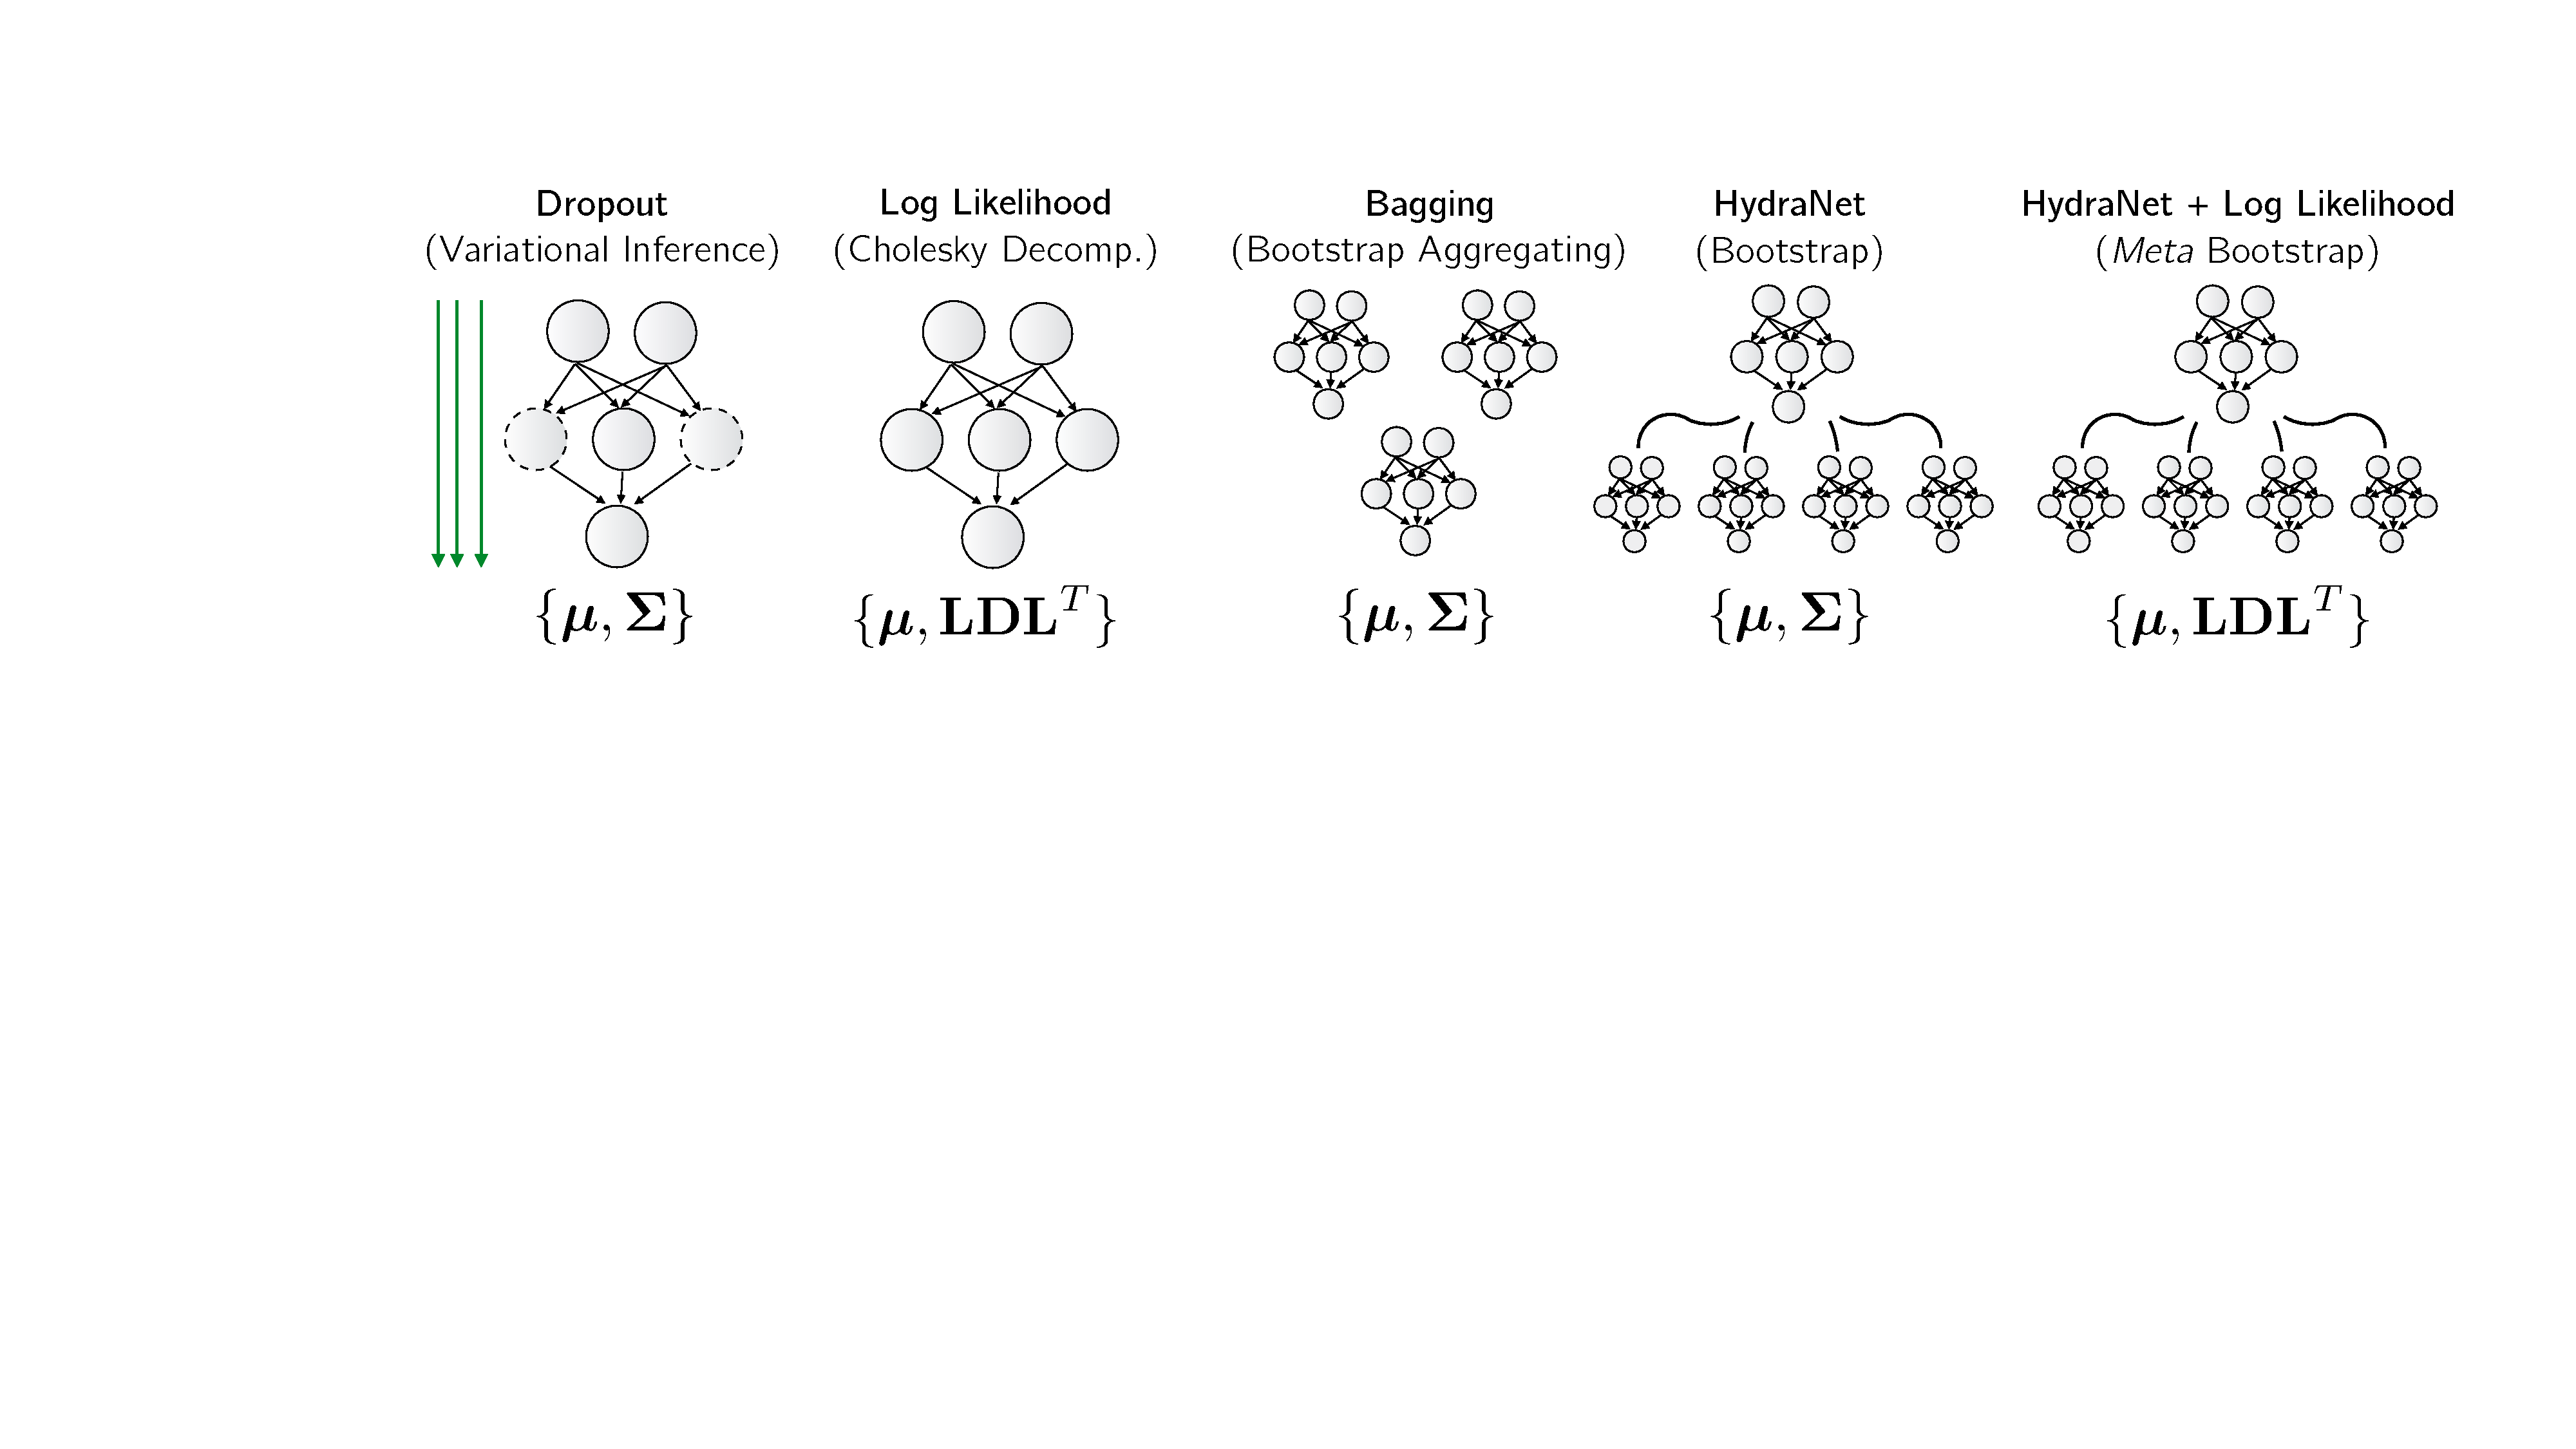
\includegraphics[width=0.95\textwidth]{lkf/nn_uncertainty.pdf}
    \caption{Different proposed uncertainty schemes for deep networks.}
    \label{fig:lkf_nn_uncertainty}    
    \end{subfigure}
    
    \begin{subfigure}[]{0.9\textwidth}
    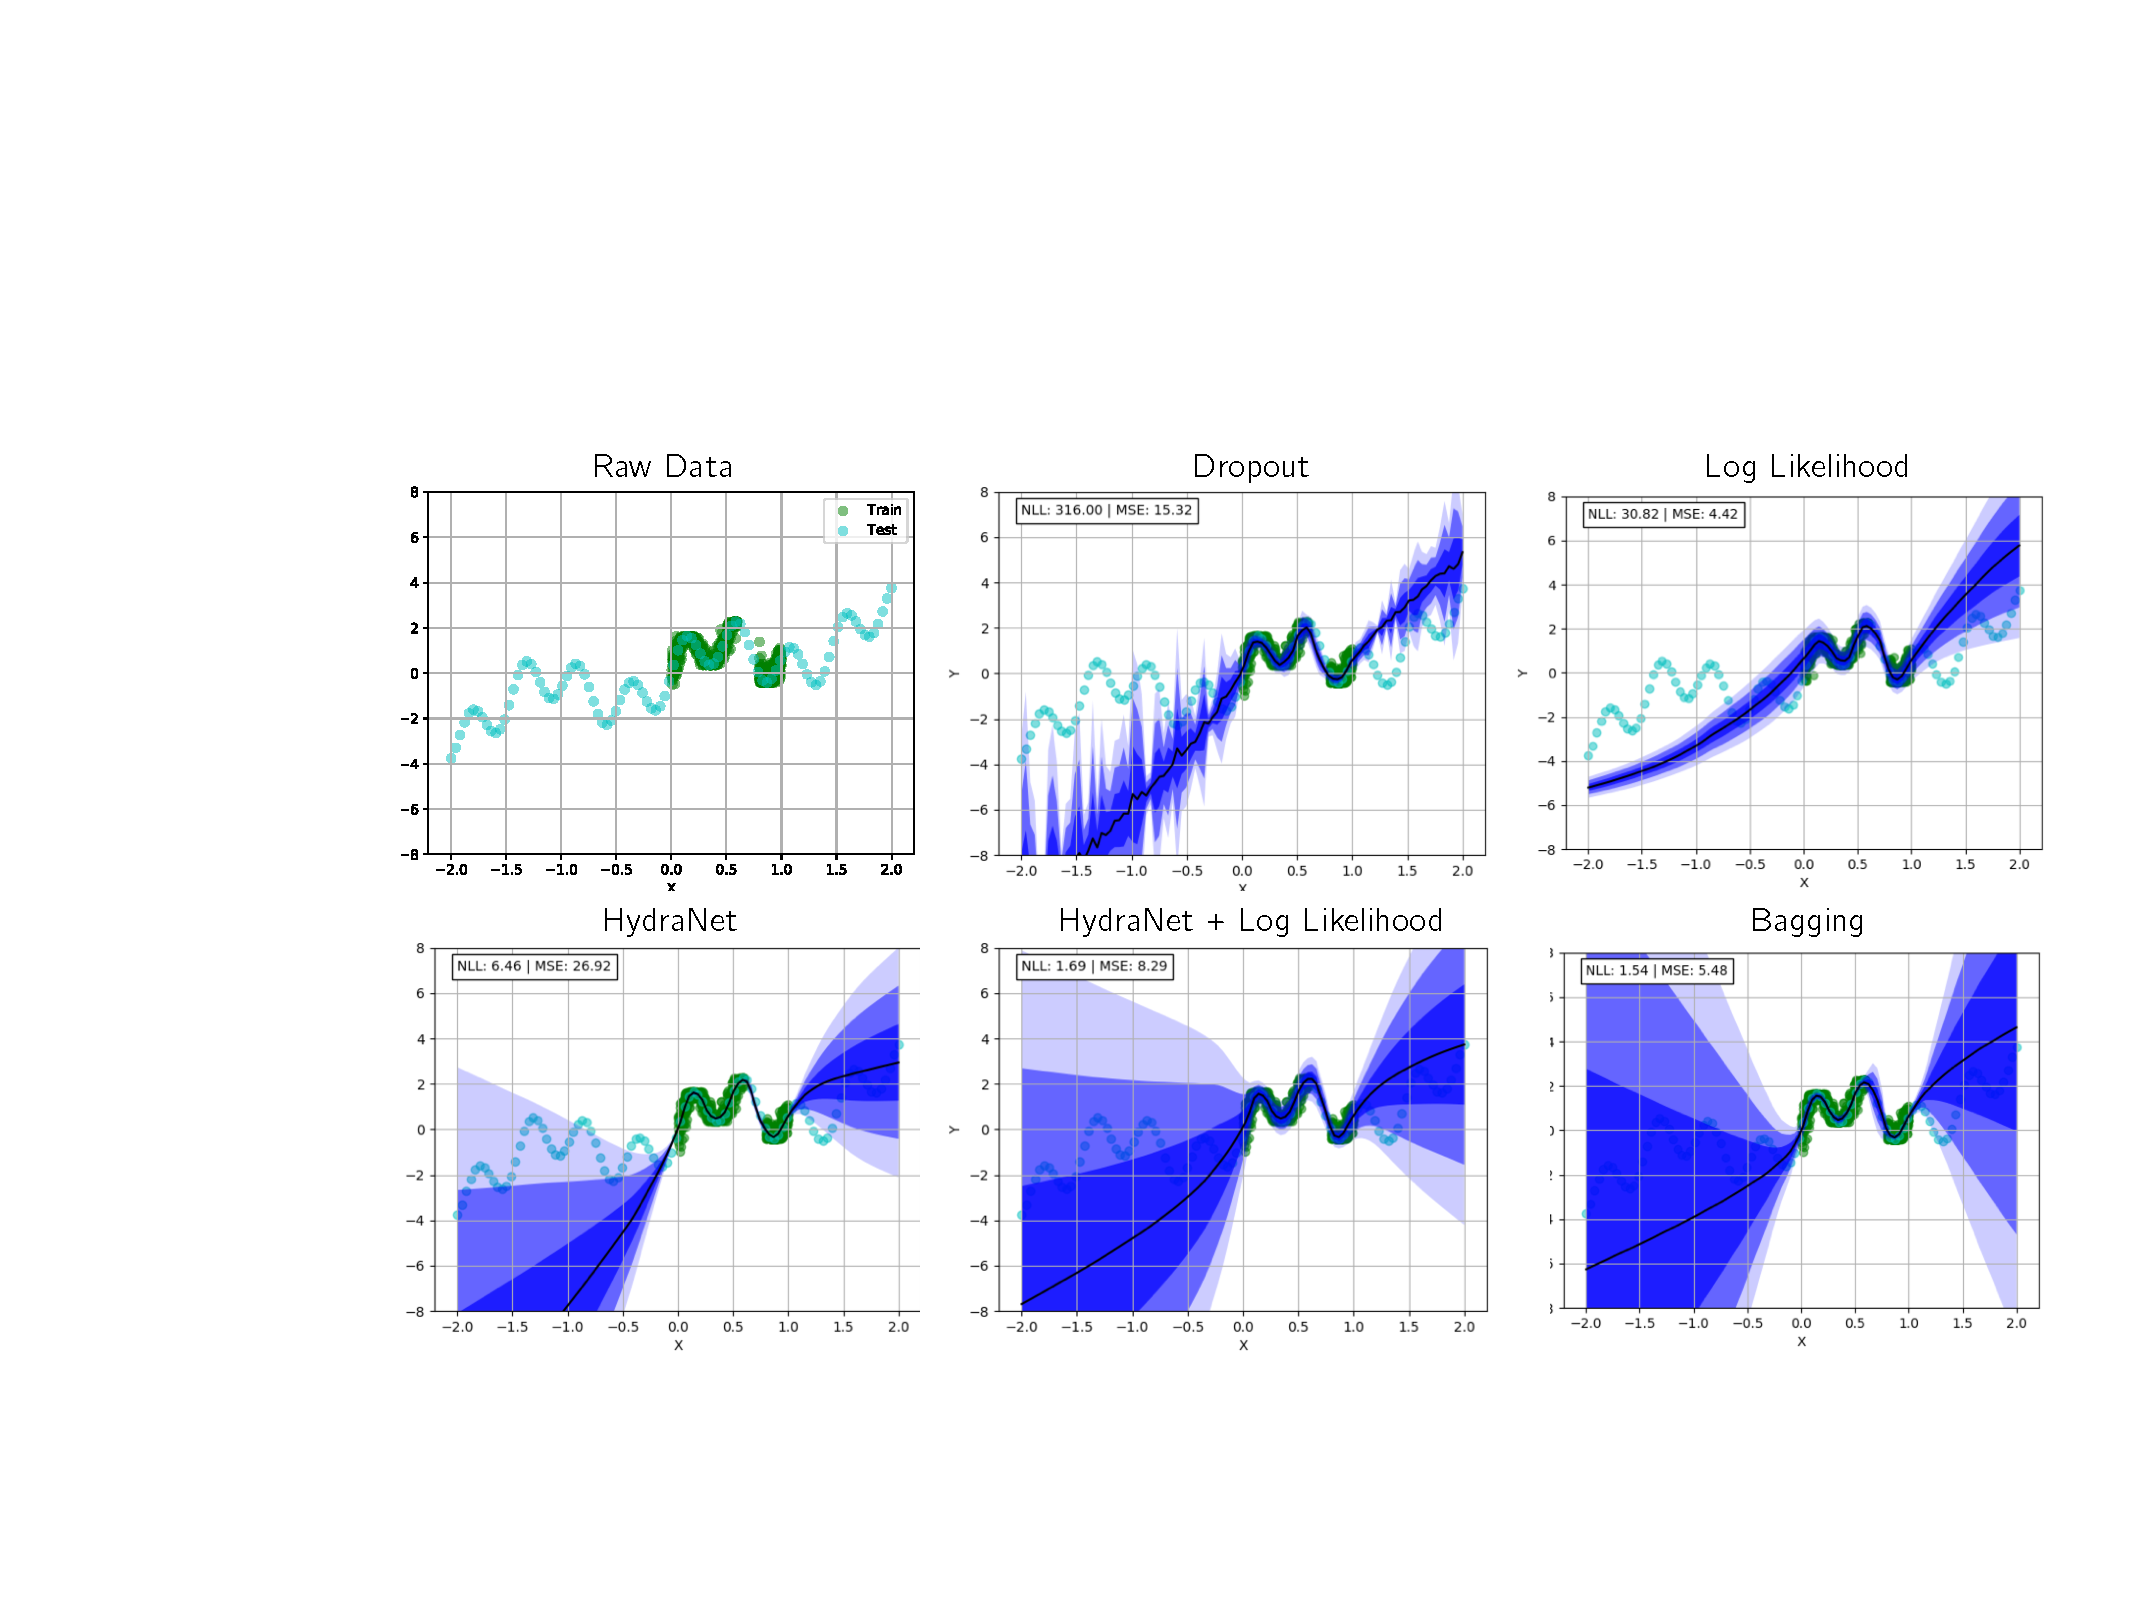
\includegraphics[width=0.95\textwidth]{lkf/uncertainty_comp.pdf}
    \caption{Comparisons of uncertainty predictions from five different probabilistic neural networks. Shades of blue represent multiples of $\sigma$. Training and test data come from the generating function $y = x + \sin{(\alpha x)} + \sin{(\beta x)}$.}
	\end{subfigure}
	\label{fig:lkf_deep-uncertainty}
	\caption{Investigations into uncertainty with deep neural networks. The network consists of two layers, with one dimensional inputs and outputs. Bagging uses 10 models and HydraNet uses 10 heads.}
\end{figure}

\begin{figure}
	\centering
	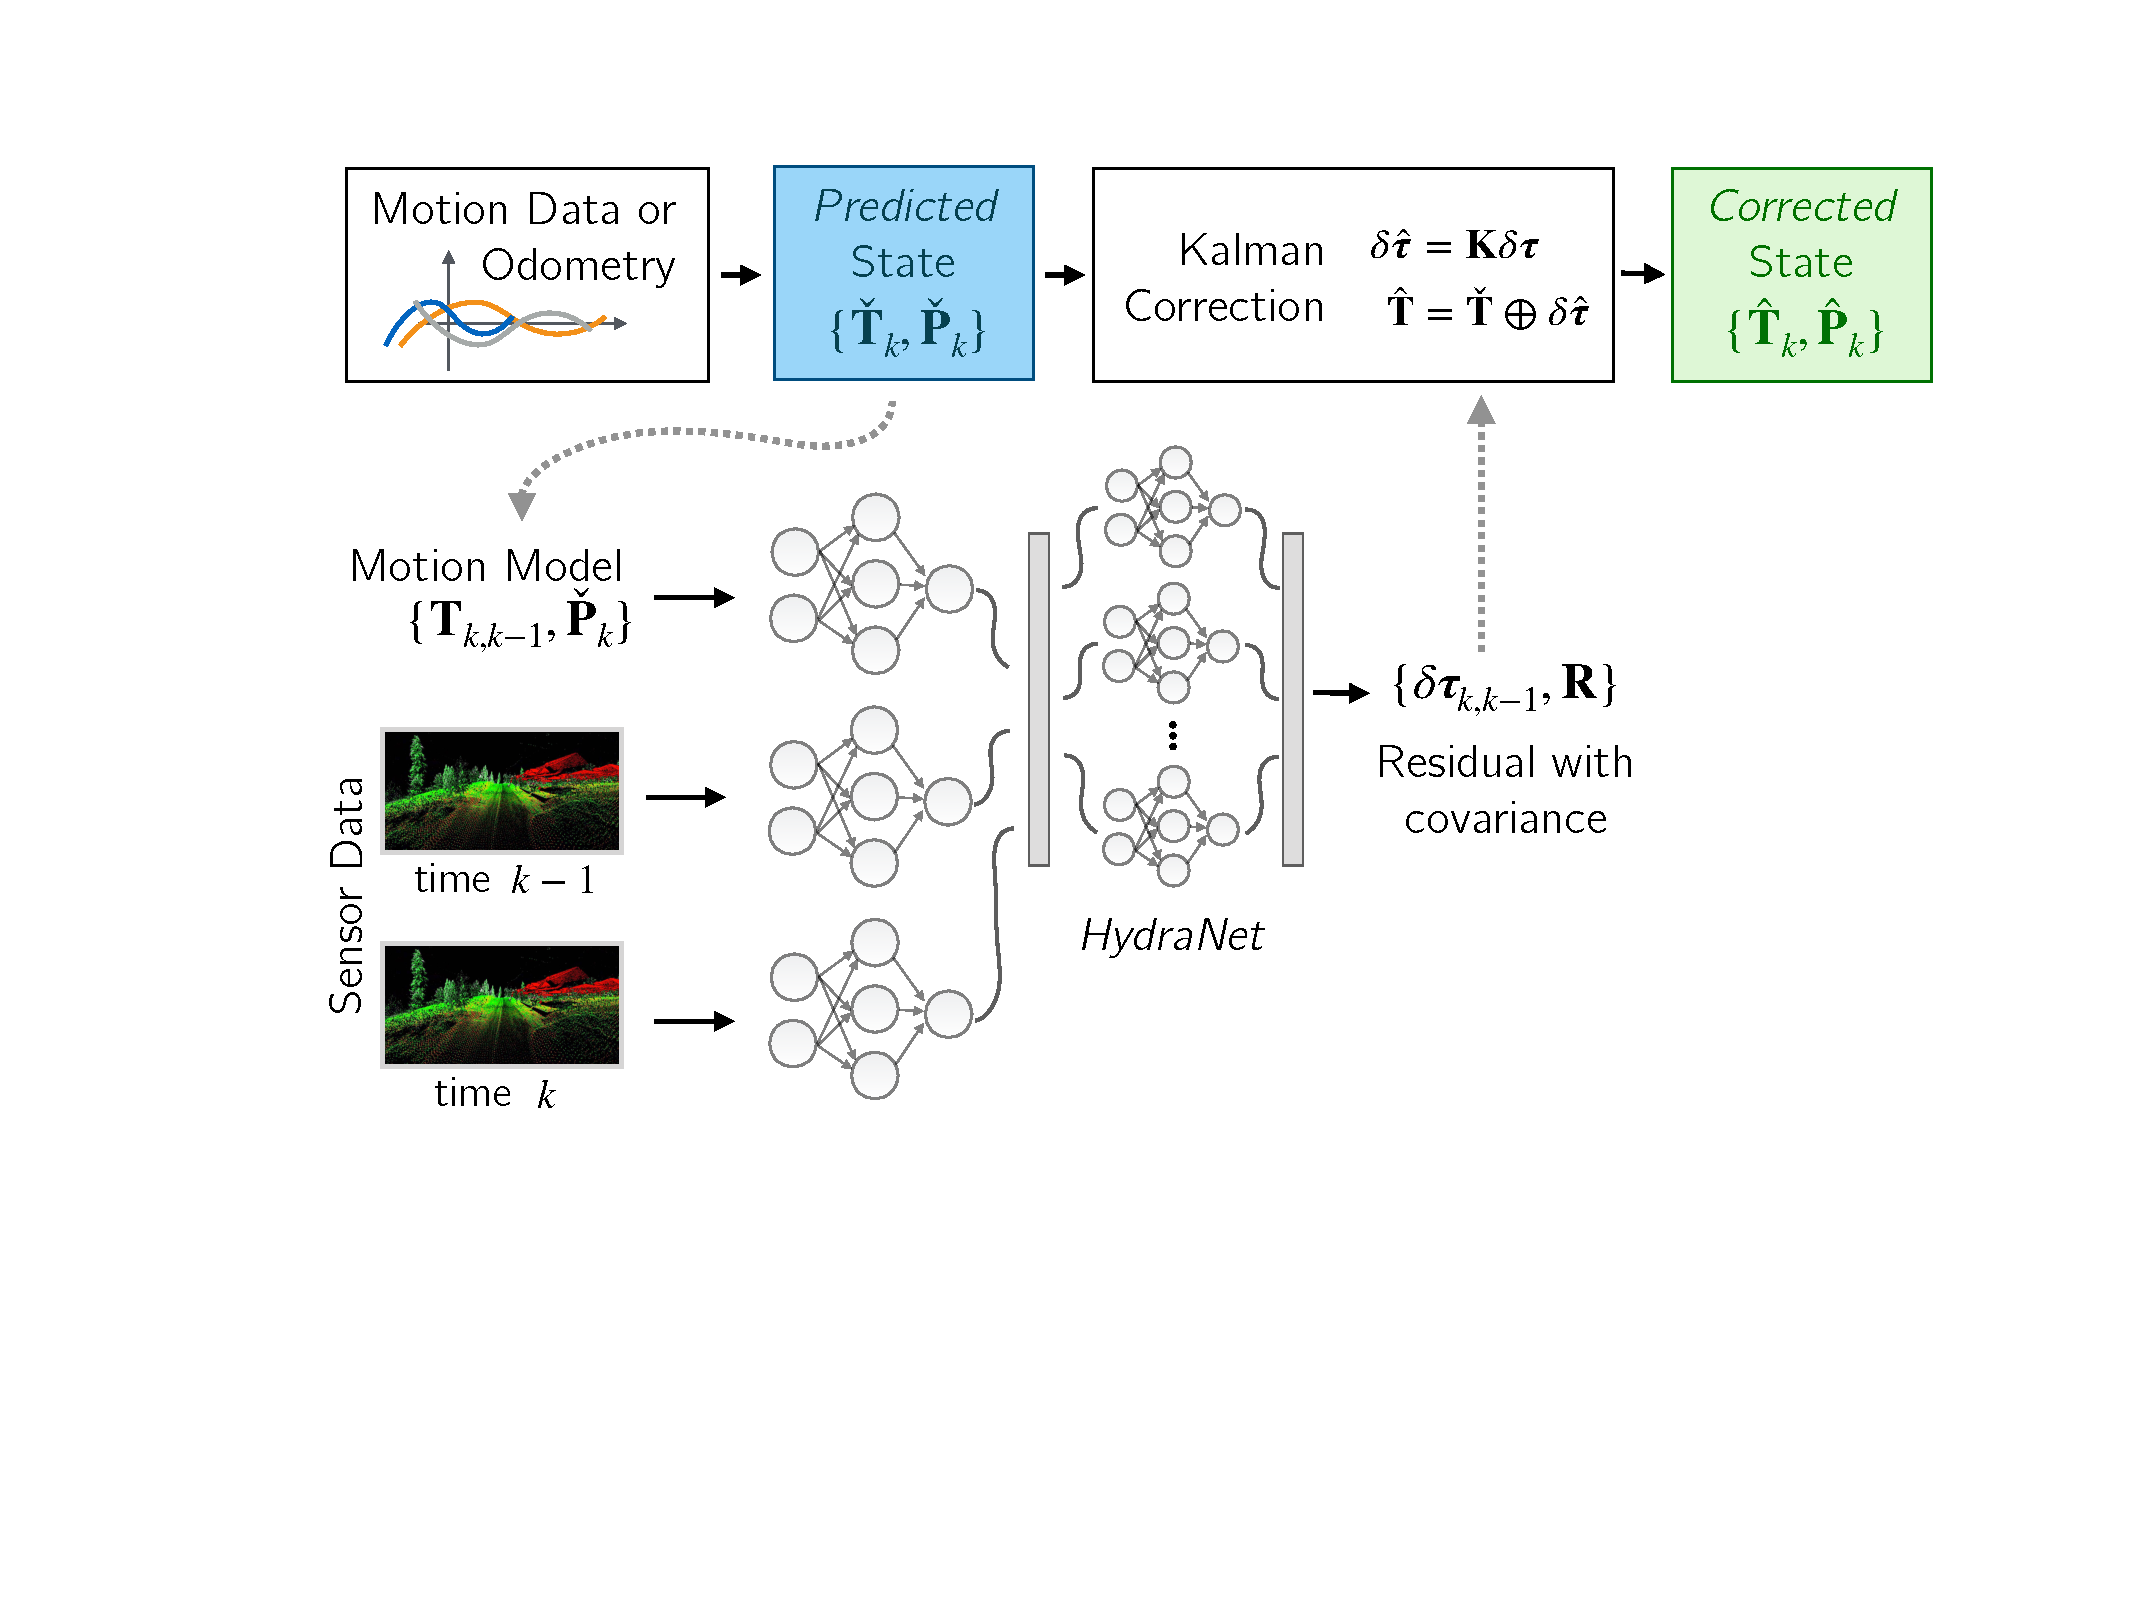
\includegraphics[width=0.9\textwidth]{lkf/rel_system}
	\caption{We present a novel way to train deep probabilistic measurement models with sparse ground truth data. Our architecture uses a multi-headed network we call a HydraNet to output residuals to a predicted state given sensor data and the state itself.}
	\label{fig:lkf_system}
\end{figure}

 